\documentclass{ecai2014}
\usepackage{graphicx, latexsym, epstopdf, setspace, units, pgfplots, helvet, times, amsmath, mathtools}
\usepackage[algo2e, noend, noline, linesnumbered]{algorithm2e}
\DontPrintSemicolon
\newcommand\todo[1]{\textcolor{red}{#1}}
\newcommand{\pushline}{\Indp}% Indent
\newcommand{\popline}{\Indm}
\newcommand{\sgn}{\mathop{\mathrm{sgn}}}
\newcommand{\tuple}[1]{\ensuremath{\left \langle #1 \right \rangle }}
\newcommand{\node}[1]{{\fontfamily{phv}\selectfont#1}}
\newcommand{\E}[1]{\mathrm{E}\left( #1 \right)}
\newcommand{\Var}[1]{\mathrm{Var}\left( #1 \right)}
\newcommand{\Cov}[1]{\mathrm{Cov}\left( #1 \right)}
\newcommand{\Corr}[1]{\mathrm{Corr}\left( #1 \right)}
\newcommand{\defeq}{\vcentcolon=}
\pgfplotsset{compat=1.9}
\setlength{\belowcaptionskip}{-15pt}
\ecaisubmission   % inserts page numbers. Use only for submission of paper.
                  % Do NOT use for camera-ready version of paper.

\begin{document}

\title{Quality-based Rewards for \\ Monte-Carlo Tree Search Simulations}

%\author{Tom Pepels \and Marc Lanctot \and Mark~H.~M. Winands \institute{Maastricht University, Department of Knowledge Engineering, Maastricht, The Netherlands, email: \{tom.pepels,marc.lanctot,m.winands\}@maastrichtuniversity.nl} }

\maketitle
\bibliographystyle{ecai2014}

\begin{abstract}
Monte-Carlo Tree Search is a best-first search technique based on sampling the state space of a given domain. In gameplay, positions are scored based on the rewards of numerous randomized play-outs. Generally, play-out rewards are defined discretely, e.g. $r \in \{-1, 0, 1\}$ and backpropagated from the expanded leaf to the root node. However, a play-out may provide additional information beside the loss/draw/win state of the terminal position. Therefore, we introduce measures for assessing the a posteriori quality of Monte-Carlo simulations. We show that altering the rewards of simulated play-outs based on their assessed quality improves results in five distinct two-player games. To achieve these results we propose two enhancements, the \emph{Relative Bonus} and \emph{Qualitative Bonus}. Both are defined as control variates, a variance reduction technique. The former is based on the number of moves made during a simulation, whereas the latter relies on a domain-dependent assessment of the game's terminal state. The proposed enhancements lead to a performance increase in all five domains discussed.
\end{abstract}

%-------------------------------------------------------------------
\section{INTRODUCTION}
\label{sec:intro}
Monte-Carlo Tree Search (MCTS) is a search method based on random sampling of a domain \cite{coulom2007efficient,kocsis2006bandit}. MCTS grows a search tree online by selecting nodes to expand based on a selection policy. Rewards stored at nodes are averaged over the results of numerous simulations. Each simulation consist of two parts, 1) the selection step, where moves are selected and played according to the a selection policy, and 2) the play-out step, where moves are played according to a simulation policy. At the end of each play-out a terminal state is reached and the result $r$, usually expressed numerically in some discrete range, e.g. $r \in \{-1, 0, 1\}$ representing a loss, draw or win, respectively, is backpropagated along the tree from the expanded leaf to the root node. All rewards are colleced at the nodes on the first ply, on which the final move to play is based. The move is selected based on either the node with the highest number of visits, the highest average reward, or a combination \cite{chaslot2008progressive}. In this paper, two techniques are proposed for determining the quality of a simulation based on the play-out sampled. The first enhancement proposed, assesses the quality of a simulation based on its length $d$. The second enhancement considers a quality assessment of the terminal state $q$. Moreover, we show that adjusting $r$ in a specific way using  $d$ or $q$ leads to increased performance in five distinct two-player games.

Other techniques for rewarding simulations have been proposed \cite{Winands2011}, where play-outs are cut-off early and their state heuristically evaluated. Furthermore, evaluating the final \emph{score} of a game has shown to improve results in games that base the winning player on the one with the highest score \cite{shibahara2008combining}. However, for some domains a heuristic evaluation may not be available or too time-consuming, and certainly not all games determine the winning player on the highest scoring player. Nonetheless, using the straightforward discrete reward $r$, any information other than the win/loss/draw state of the play-out's final position is disregarded. For these reasons, we propose assessing the rewards of play-outs based on any information available at the terminal state.

The paper is structured as follows. First, the general MCTS framework is discussed in Section \ref{sec:mcts}. Next, in Section \ref{sec:poqual}, two different techniques for assessing the quality of play-outs are detailed. Section \ref{sec:qoreward} explains how rewards can be altered given using the quality measures from the previous section. Followed by pseudo-code outlining the proposed algorithm. Finally the performance of the proposed enhancements is determined in Section \ref{sec:experiments}, accompanied by a discussion and conclusion.

%-------------------------------------------------------------------
\section{MONTE-CARLO TREE SEARCH}
\label{sec:mcts}
\begin{figure}[ht]
	\centering
	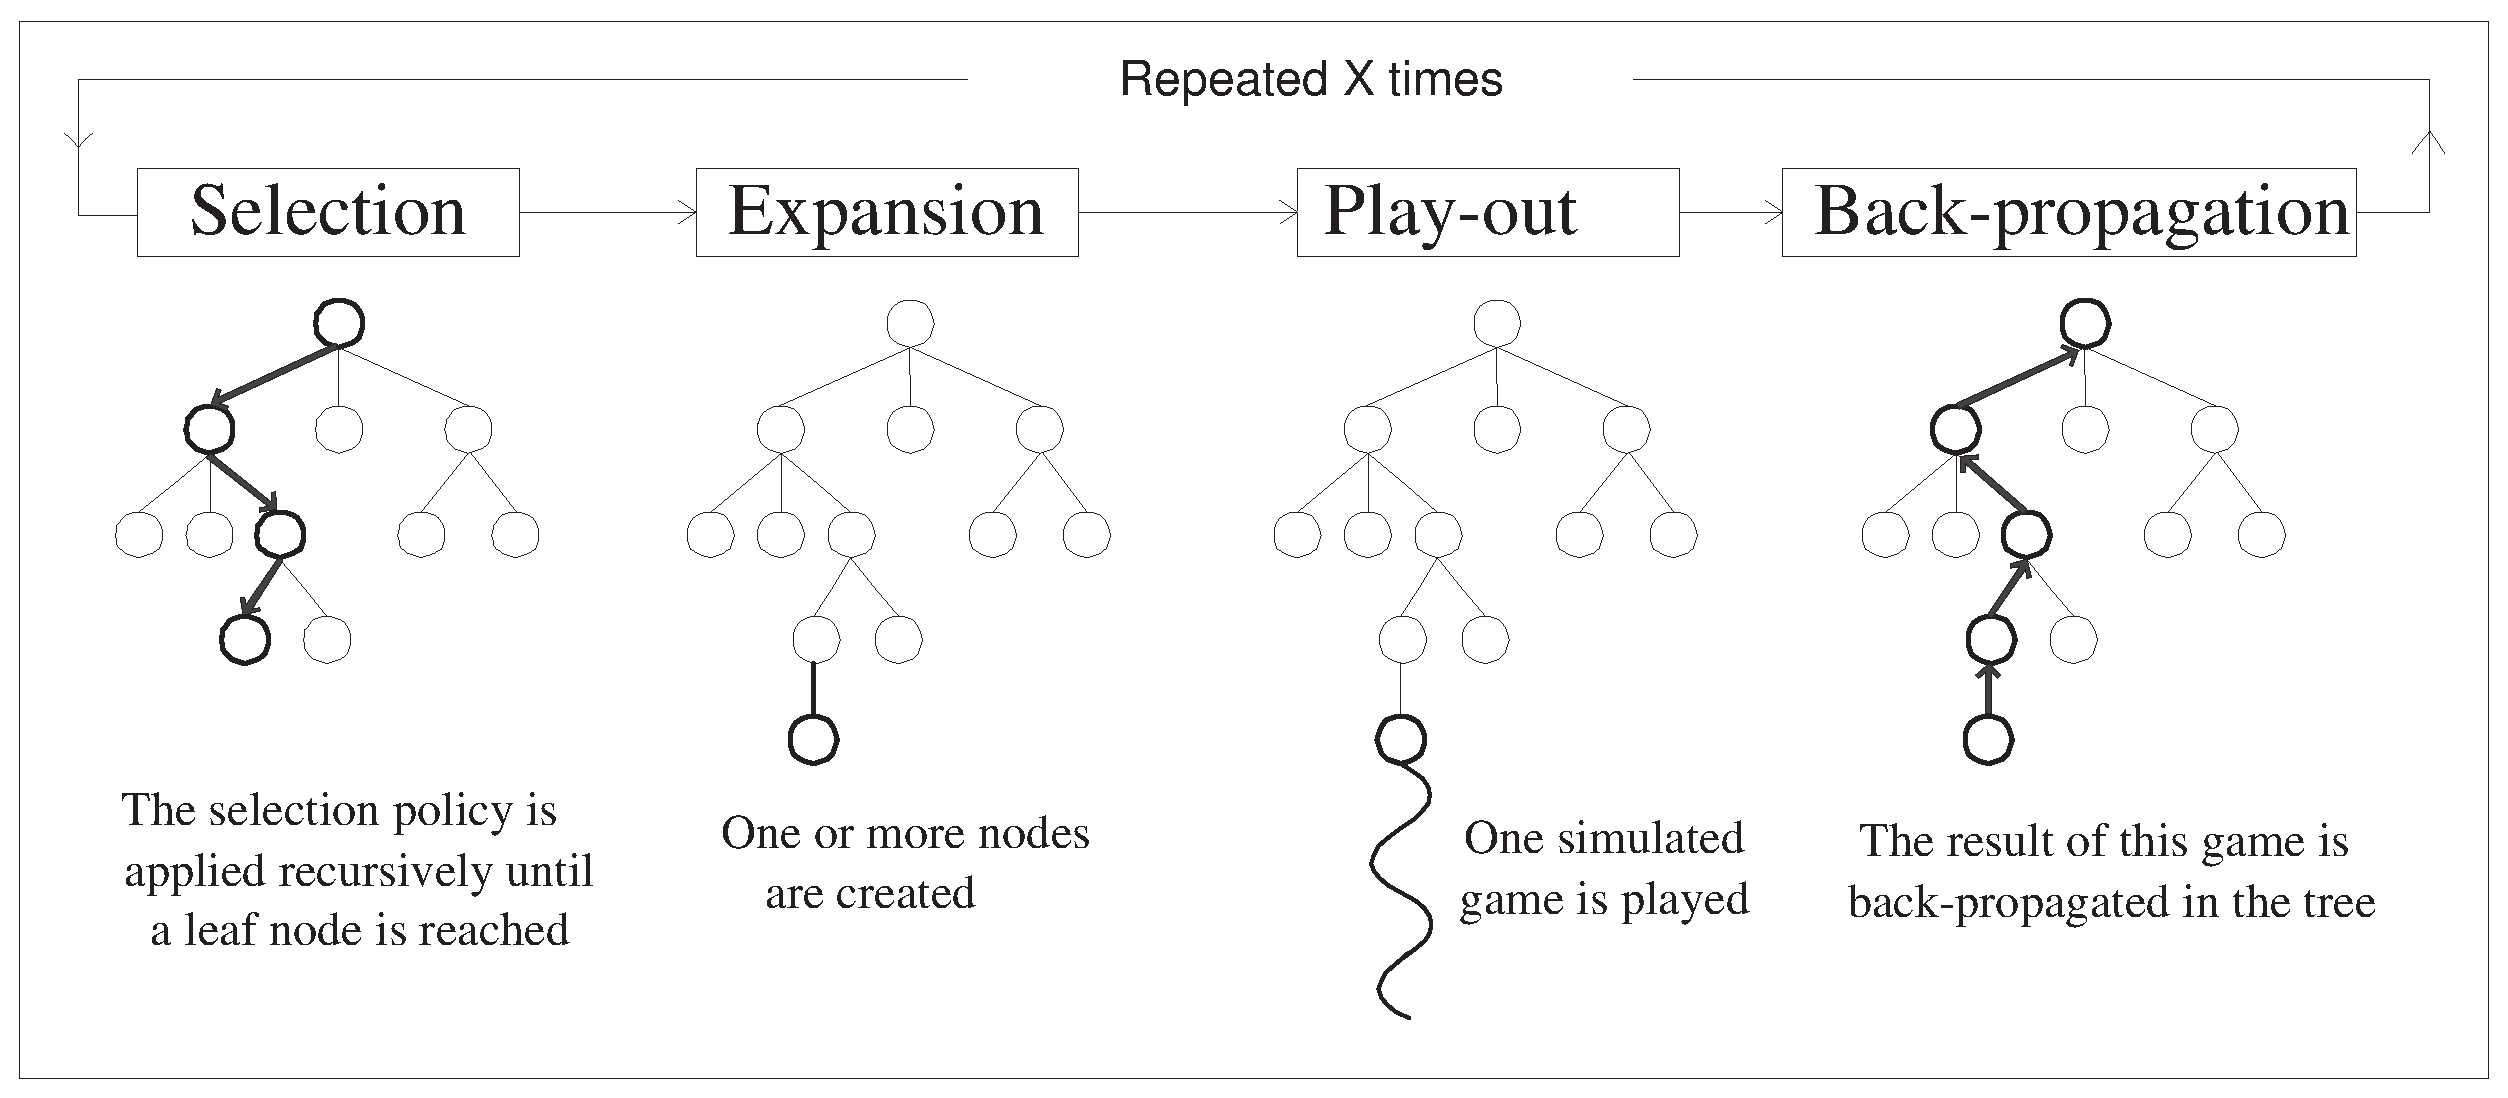
\includegraphics[width=.45\textwidth]{img/figure1.eps}
	\caption{Strategic steps of Monte-Carlo Tree Search \cite{chaslot2008progressive}.}
	\label{fig:mcts-algorithm}
\end{figure}
%from pac-man paper
Monte-Carlo Tree Search (MCTS) is a best-first search technique based on random sampling of the state space for a specified domain \cite{coulom2007efficient,kocsis2006bandit}. In gameplay, this means that decisions are made based on the results of random play-outs. MCTS has been successfully applied to various two-player games games such as Go \cite{lee2010current}, Lines of Action \cite{Winands2010b}, and Hex \cite{arneson2010monte}. Moreover, MCTS has recently seen successes in other domains such as real-time strategy games \cite{browne2012survey}, arcade games such as Ms Pac-Man \cite{enhancementspacmancig12} and the Physical Travelling Salesman problem \cite{powleytsp}, but also in real-life domains such as optimization, scheduling and security \cite{browne2012survey}.

In MCTS, a tree is built incrementally over time and maintains statistics at each node corresponding the rewards collected at those nodes and number of times the nodes have been visited. The root of this tree corresponds to the agent's current position. The basic version of MCTS consists of four steps, which are performed iteratively until a computational threshold is reached, i.e. a set number of iterations, an upper limit on memory usage, or a time constraint. The four steps (depicted in Figure \ref{fig:mcts-algorithm}) at each iteration are \cite{chaslot2008progressive}:
\begin{itemize}
\item {\bf Selection.} Starting at the root node, children are chosen according to a selection policy (described in Subsection \ref{subsec:uct}). When a leaf node is reached that does not represent a terminal state it is selected for expansion.
\item {\bf Expansion.} All children are added to the selected leaf node given available moves.
\item {\bf Play-out.} A simulated play-out is run, starting from the state of the added node. Moves are performed randomly or according to a simulation policy until a terminal state is reached.
\item {\bf Backpropagation.} The result of the simulated play-out is propagated immediately from the selected node back up to the root node. Statistics are updated along the tree for each node selected during the selection step and visit counts are increased.
\end{itemize}
The combination of moves selected during the selection and play-out steps form a single simulation. In its basic form, MCTS requires no evaluation function. Nonetheless, in most cases it is beneficial to add some domain knowledge for selecting moves to play during play-out. MCTS can be terminated anytime and select a move to play based on the rewards and visits collected on the first ply.
% /from pac-man paper

%-------------------------------------------------------------------
\subsection{UCT}
\label{subsec:uct}
%from pac-man paper
During the selection step, a policy is required to explore the tree for rewarding decisions and finally converge to the most rewarding one. The Upper Confidence Bound applied to Trees (UCT) \cite{kocsis2006bandit} is derived from the UCB1 policy \cite{auer2002using} for maximizing the rewards of a multi-armed bandit. UCT balances the exploitation of rewarding nodes whilst allowing exploration of lesser visited nodes. Consider a node $p$ with children $I(p)$, then the policy determining which child $i$ to select:
\begin{equation}
\label{eq:uct}
i^* = argmax_{i \in I(p)}\left\{ v_i + C \sqrt{ \frac{\ln{n_p}}{n_i}}\right\}
\end{equation}
where $v_i$ is the score of the child $i$ based on the average result of simulations that visited it. $n_p$ is the visit count of the node and $n_i$ the visit count of the current child. $C$ is the exploration constant to be determined by experimentation.
% /from pac-man paper

\section{ASSESSING SIMULATION QUALITY}
\label{sec:poqual}

In this section two measures by which the quality of the terminal state of a simulation can be assessed are discussed. First, the length of a simulation is detailed as a quality measure, second, a heuristic assessment of terminal states is considered. In the next section we establish how these techniques can be used to enhance the rewards of MCTS simulations.

The first, straightforward assessment of a simulation's quality is the length of the game played. Consider a single MCTS simulation as depicted in Figure \ref{fig:mcts-simulation}, here we can define two seperate distances: 
\begin{enumerate}
\item The number of nodes between the root node \node{S} to the expanded leaf \node{N}, $d_{SN}$,
\item The number of moves required to reach \node{T}, the simulation's terminal state, from \node{N} during play-out $d_{NT}$.
\end{enumerate}
The length of the simulation is then defined as the sum of these distances:
\begin{equation}
d = d_{SN} + d_{NT}
\label{eq:m_ST}
\end{equation}
i.e. the total number of moves made by both players before reaching the terminal state of the game \node{T} from \node{S}, the root's game state.

\begin{figure}[t]
	\centering
	\includegraphics[width=.3\textwidth]{img/figure2_new.png}
	\caption{A single MCTS simulation \cite{finnsson2010learning}.}
	\label{fig:mcts-simulation}
\end{figure}

Moves selected during play-out are generated by some simulation strategy. Generally this either a random strategy, or a rule-based, reactive strategy, combined with a source of randomness such as an $\epsilon$-greedy selection \cite{sturtevant2008analysis,sutton1998reinforcement}. Various alternative methods have been proposed, such as using low-level $\alpha\beta$ searches \cite{Winands2011}, and methods that learn a strategy online, such as N-Grams and the Last-Good-Reply policy \cite{Tak2012}, or the Move-average Sampling Technique (MAST) \cite{finnsson2008simulation}. However, each of these methods and strategies have some random element in common. Moreover, they select moves that are far from optimal, because they have to make quick decisions to allow for numerous simulations to be made during the allowed time. As such, each move played ultimately increases uncertainty with respect to the accuracy of the final result by some degree. Hence, the length of the simulation may be regarded as an indicator of the accuracy of its result.

The main benefit of using simulation length as a quality measure is that it is domain independent. Unless the game's length is fixed, the variance of the length of a play-out in particular can be informative in determining its quality. Moreover, in certain games such as Chinese Checkers, simulation length has been considered part of the evaluation function \cite{roschke2013cc}.

The second measure of a simulation's quality is based on a heuristic assessment of the game's terminal state. Although evaluation functions can be designed for most games, they're used to evaluate non-terminal states and assign them a specific value. However, MCTS generally performs a play-out until a terminal state is reached. Therefore, we are interested in assessing the terminal state of a game rather than intermediary states. This leaves potentially less informative features to be evaluated, yet provides a direct application to MCTS.

As before, consider a single MCTS simulation as depicted in Figure \ref{fig:mcts-simulation}. When a terminal state is reached, a quality assessment function is called to evaluate the position with respect to the winning player. This measure $q \in (0, 1)$ should reflect the quality of a terminal state. For instance, in a game with material such as Breakthrough, Chess or Checkers, an evaluation can be based on scoring the remaining material of the winning player. For a racing game such as Chinese Checkers, the inverse of the number of pieces the opponent has in his target base can be considered. As such, the quality is based on the a posteriori evaluation of the terminal state. Having witnessed the states and actions performed from \node{S} to \node{T}, the score is based on an assessment of \node{T} given the progression \node{S} \ldots \node{N} \ldots \node{T} (see Figure \ref{fig:mcts-simulation}).

%-------------------------------------------------------------------
\section{QUALITY-BASED SIMULATION REWARDS}
\label{sec:qoreward}
Based on the classification of quality measures in the previous section, we propose two reward alterations for MCTS: \emph{Relative Bonus} and the \emph{Qualitative Bonus}, relating to the length of simulations and the quality assessment of terminal states, respectively. 

In the proposed framework, MCTS simulations return a tuple of four reward values, $\tuple{r,\tau,q,d_{NT}}$ representing the outcome $r\in~\{-1, 0, 1\}$, the winning player $\tau$, the quality assessment of the terminal state $q$, and the distance from the expanded node \node{N} to the terminal state \node{T}, $d_{NT}$, respectively. $d$ is then computed as shown in Equation \ref{eq:m_ST}. In the first subsection the Relative Bonus (RB) is defined, based on the value of $d$. The following subsection details the Qualitative Bonus (QB), which is similar to RB and is based on the value of $q$.

\subsection{Control Variates}
Variance reduction methods in mathematical simulation are used to improve estimates by reducing the variance in a simulation's output \cite{kelton2000simulation}. Recently, using variance reduction techniques for MCTS has been proposed by Veness et. al. \cite{Veness11variance}. They applied, among others, control variates to UCT in different stochastic games to improve results by the reduction of variance in the reward signal. \todo{Say how our approach differs from theirs.}

Control variates (CV) take advantage of a possible correlation between two random variables $X$ and $Y$, to improve the estimate $\E{X}$ given that the mean $v=\E{Y}$ is known. This is achieved by adding the deviation of $Y$ from its mean, scaled by a constant $a$, to $X$. Which results in a new, controlled estimator $Z\defeq X+a\left(Y-v\right)$. For $a$, one can derive an optimal constant $a^*=-\Cov{X,Y}\mathbin{/}\Var{Y}$ such that the reduction in variance is optimal.

Let $\rho$ be the player for which the current search is run, and $X$ the simulation output, i.e. the reward resulting from MCTS simulations such that:
\begin{equation}
  \bar{X}_n=
  \begin{cases}
    $1$ 	& \text{if $\rho$ wins the play-out},\\
    $-1$ 	& \text{otherwise}
  \end{cases}
\end{equation}
Next, we define $Y$ as as one of the quality measures discussed in Section \ref{sec:poqual}, $Y_n=d$ or $Y_n=q$. Assuming that $X$ and $Y$ are correlated, i.e. $\Corr{X,Y}\neq0$, we can find an optimal $a*$ such that variance in the reward will be reduced. However, since we have no clear means of determining $v$, $\Cov{X,Y}$, or $\Var{Y}$ we propose to use appropriate estimators for these quantities. Moreover, particularly in the case of RB, $X$ and $Y$ have quite different ranges, which leads to numerical problems when computing $a*$. We therefore propose to use normalized and standardized measures for $Y$. Note that, although we expect that reducing the variance in the reward signal benefits performance, it is not a guarantee. Moreover, it is possible that a larger performance increase is gained by using a non-optimal $a*$, as our quality measures may provide more benefits than variance reduction alone.

\subsection{Relative Bonus}
\label{subsec:rb}
First, note that $d$ depends considerably on both the domain and the progress of the game. By itself, the variable is neither normalized, nor relative to a central tendency over time. As such, adding the value to $r$ as is, leads to a biased distribution of the value over time, where, at the beginning of a game, $d$ takes on higher values than when the game nears its end. Moreover, considering that the length of a game cannot be determined beforehand, we have no accurate way of normalizing the observed values absolutely, based on the expected total length of the game. Therefore, two normalizers are to be approximated: 1) a central measure, to relate the desired variable to the current game's progress, and 2) a normalizing distance to the central measure, since the variance of observed $d$ values may also differ over time.

A central measure can be approximated online, by maintaining an average $\bar{D}^\tau$ for each player (indexed by $\tau$), over the distribution of observed $d$ values $D$. After each simulation ends, $d$ is compared to $\bar{D}^\tau$.
\begin{equation}
\delta_d = \bar{D}^\tau - d
\end{equation}
After each simulation, $\bar{D}^\tau$ is updated with the observed $d$. This ensures $\delta_d$ is relative to the current progress of the game, and independent of the domain's tendency regarding the length of games. Moreover we achieve the desired effect of valuating simulations shorter than average with a positive value, and longer ones with a negative value. However, $\delta_d$ is still dependent on the progress of the game. In most domains, the start of any game will have a high variance with respect to the length of simulations. Insufficient prior moves have been made and therefore, MCTS can not yet accurately predict the progression of the game. As a consequence, play-outs last longer at the start of the game than when the endgame is reached. Intrinsically, the variance of the observed $d$ values over time may differ substantially. Which leads to the requirement of a normalizer.

$\hat{\sigma}^\tau_D$ is the sample standard deviation of the distribution $D$, which can be used to normalize $\delta_d$ with respect to the current variance of the length of simulated games. Now we can define a normalized variable $\lambda$ as follows:

\begin{equation}
\lambda = \frac{\delta_d}{\hat{\sigma}^\tau_D}
\end{equation}

Now, $\lambda$ is both normalized with the sample standard deviation, and is relative to $\bar{D}^\tau$. This means $\lambda$ is both independent of the progress of the game, and normalized with respect to the current variance in the length of simulations. In fact, $\lambda$ is a \emph{student's t} statistic, which estimates the number of standard deviations that $\delta_d$ is removed from the current sample mean. 

Using an estimated mean may cause the search to be biased, i.e. moving into the direction of faster games. A possible solution to this problem is to reset $\bar{D}^\tau$ and $\hat{\sigma}^\tau_D$ in between moves. Moreover, rewards of the first 100 simulations are not altered.

Since the distribution of $D$ is not known, $\lambda$ can still take on unrestricted values, particularly if $D$ is skewed, or has long tails. Moreover, the relation with the desired reward is not neccesarily linear. As such, in order to both bound, and shape the values of the bonus $b(\lambda)$ we propose to use a sigmoid function centered around $0$ on both axes, and with a range of $[-0.25, 0.25]$. This range is a best-guess of the value of $a*$ discussed in the previous subsection. Any method for computing $a*$ either off-line or on-line may result in increased performance depending on the domain.

\begin{equation}
b(\lambda)=-0.25+\frac{1}{2\left(1+e^{-k\lambda}\right)}
\label{eq:sigmoid}
\end{equation}

%Figure \ref{fig:sigmoids} shows the graphs for three different values of $k$ in Equation \ref{eq:sigmoid}. 
$k$ is a constant to be determined by experimentation, which shapes the bonus to be added to $r$. Higher values of $k$ determine both the steepness, and the start and end of the horizontal asymptotes of the sigmoid function.

%\begin{figure}[h]
%\centering
%\begin{tikzpicture}[scale=0.6]
%  \begin{axis}[
%	ylabel = Bonus $b(\lambda)$,
%    xlabel = Normalized distance to mean $\lambda$,
%  	axis equal image=false 
%  	]

 %   \addplot[red, mark=none, domain =-3:3] {1/(2*(1+e^(-x)))) - .25} node [pos=0.8,pin={-10:$k=1$},inner sep=0pt]{};
 %   \addplot[orange, mark=none, domain =-3:3] {1/(2*(1+e^(-1.5*x))) - .25} node [pos=0.6,pin={-10:$k=1.5$},inner sep=0pt]{};
 %   \addplot[blue, mark=none, domain =-3:3] {1/(2*(1+e^(-2*x))) - .25} node [pos=0.7,pin={-200:$k=2$},inner sep=0pt]{};
 %      \addplot[purple, mark=none, domain =-3:3] {1/(2*(1+e^(-2.5*x))) - .25} node [pos=0.6,pin={-200:$k=2.5$},inner sep=0pt]{};
 %   \draw[ultra thin] (axis cs:\pgfkeysvalueof{/pgfplots/xmin},0) -- (axis cs:\pgfkeysvalueof{/pgfplots/xmax},0);
%	\draw[ultra thin] (axis cs:0,\pgfkeysvalueof{/pgfplots/ymin}) -- (axis cs:0,\pgfkeysvalueof{/pgfplots/ymax}); 
%  \end{axis}
%\end{tikzpicture}
%    \caption{Bonusses resulting from different $k$ constants in Equation \ref{eq:sigmoid}.}
%	\label{fig:sigmoids}
%\end{figure}

Finally, the reward $r$ returned by the original simulation is altered by $b(\lambda)$ as follows:
\begin{equation}
r_b = r + \sgn(r) \times b(\lambda)
\end{equation}

This value is backpropagated from the expanded leaf to the root node. The range of $r_b$ is now $[-1.25, 1.25]$, i.e. the bonus $b(\lambda)$ is centered around the possible values of $r$.

\subsection{Qualitative Bonus}
\label{subsec:qb}
Calculation of the Qualitative Bonus follows the same procedure as the Relative Bonus. Similar to RB, a distribution over observed $q$ values is maintained $Q \sim \mathcal{N}(\bar{Q}, \hat{\sigma}_q)$ for each player $\tau$. The value of $q$ is determined by a domain dependent assessment of the quality of the terminal state. Assuming that higher values of $q$ represent a higher quality terminal state for the winning player $\tau$, then $\delta_q$ is:
\begin{equation}
\delta_q = q - \bar{Q}^\tau
\end{equation}
Where $\bar{Q}^\tau$ is updated with $q$ after every simulation. Consequently, $\lambda$ is redefined as:
\begin{equation}
\lambda = \frac{\delta_q}{\hat{\sigma}^\tau_Q}
\end{equation}
Finally the bonus $b(\lambda)$ is computed using the sigmoid function in equation \ref{eq:sigmoid} with an optimized $k$ constant, and summed with the result of the simulation $r$.

%-------------------------------------------------------------------
\section{PSEUDO-CODE}

\begin{algorithm2e}[ht]
\setstretch{1.15}
  {\sc mcts}(node $p$, node depth $d_{Sp}$):												\;
  \pushline
    \If{isLeaf($p$)}{Expand($p$)}
    Select a child $i$ according to Eq.~\ref{eq:uct} 										\;
    $d_{Si} \gets d_{Sp} + 1$																\; \label{alg:depth}
    \eIf{$n_i = 0$}{
    	$\tuple{r, \tau, q, d_{iT}} \gets$ Playout$(i)$ 									\; \label{alg:results}
    	$d \gets d_{Si} + d_{iT}$															\;			
    	\If{enabled$(b_r)$ and $\hat{\sigma}^\tau_D > 0$}{
    		$r \gets r + \sgn(r) \times$ BONUS$(\bar{D}^\tau - d, \hat{\sigma}^\tau_D)$ 	\; \label{alg:rb}
    		update $\bar{D}^\tau$ and $\hat{\sigma}^\tau_D$ with $d$						\; \label{alg:meanstddev}
		}
		\ElseIf{enabled$(b_q)$ and $\hat{\sigma}^\tau_Q > 0$} {
    		$r \gets r + \sgn(r) \times$ BONUS$(q -\bar{Q}^\tau, \hat{\sigma}^\tau_Q)$ 		\; \label{alg:qb}
    		update $\bar{Q^\tau}$ and $\hat{\sigma}^\tau_Q$ with $q$ 						\;
    	}
    	update node $i$ with $r$															\;
    }{
    	$r \gets$ -{\sc mcts}($i$, $d_{Si})$)												\; 
    }
    update node $p$ with $r$																\;
   \popline
    {\bf return} $r$																		\;
  																							\;
    {\sc bonus}(offset from mean $\delta$, sample std. dev. $\hat{\sigma}$):				\;	\label{alg:bonus}
    \pushline
    	$\lambda \gets \nicefrac{\delta}{\hat{\sigma}}$										\;	\label{alg:lambda}
    	$b \gets -0.25 + \nicefrac{1}{2\left(1+e^{-k\lambda}\right)}$						\;	\label{alg:b}
    \popline
    \bf{return} $b$																			\;
  \vspace{0.3cm}
  \caption{Pseudo-code of the MCTS and BONUS functions \label{alg}}
\end{algorithm2e}

Algorithm~\ref{alg} summarizes a single iteration of MCTS enhanced with RB and QB. Note that negamax backups are used in this setup, and therefore $r$ is relative to the player to move at the start of the play-out. Whenever and \emph{update} is used in the algoritm, it refers to updating the average reward for a node, or the sample mean and standard deviation for $\bar{D}^\tau$ and $\bar{Q}^\tau$. During selection, starting from the root, the depth of the current node is updated on line \ref{alg:depth}. Whenever an expandable node is reached, its children are added to the tree and a play-out is initiated from one of them. A play-out returns a tuple of results, on line \ref{alg:results} 4 different values are returned: 1) the result of the play-out $r \in \{-1, 0, 1\}$, 2) the winning player $\tau$, 3) the assessed quality of the play-out's terminal state $q \in (0,1)$ defined in Subsection~\ref{sec:qoreward}, and 4) the number of moves made during play-out $d_{iT}$ defined in Subsection~\ref{sec:qoreward}. Using these values $r$ is altered. On line \ref{alg:rb} the relative bonus is applied to $r$, using the difference with the winning player's current mean $\bar{D}^\tau - d$, i.e. lower values of $d$ give a higher reward. After which the current mean and standard deviation are updated on line \ref{alg:meanstddev}. QB is applied on line \ref{alg:qb} using the assessed quality of the play-out $q$. Note that the distance to the mean is defined as $q - \bar{Q}^\tau$, because in contrast to RB, higher values of $q$ imply better results. The {\sc bonus} function on line \ref{alg:bonus}, computes the normalized $\lambda$ (line \ref{alg:lambda}) and, successively the bonus $b$ (line \ref{alg:b}) using the sigmoid function, as defined in Subsections \ref{subsec:rb} and \ref{subsec:qb}.

%-------------------------------------------------------------------
\section{EXPERIMENTS}
\label{sec:experiments}
To determine the impact on performance of RB and QB, experiments were run on 5 different two player games.

\subsection{Experimental setup}
\label{subsec:expsetup}
The proposed enhancements were tested in five distinct two player games.

{\emph Amazons} is played on a 10 x 10 chessboard. Each player has four amazons that move (and shoot) as queens in chess. However, each move consist of two parts, first the amazon moves, after which she must fire an arrow on an empty position in range, and this square on the board is blocked. The last player to move wins the game.

{\emph Breakthrough} is played on an 8 x 8 board. Each player starts with 16 pawns on one side of the board and the aim is to move one of them to the opposite side.

{\emph Cannon} is a chess-like game where the goal is to checkmate your opponents immobile town. Each player has one town he must place at the start of the game, and 15 soldiers. Soldiers can move or capture forward or may retreat if next to an opponent's soldier. Moreover, three soldiers in a row form a cannon that can move and shoot across the board.

{\emph Checkers} is played on an 8 x 8 board, and the goal is to capture all opponent's pieces.

{\emph Chinese Checkers} is played on a star shaped board. Each player starts with six pieces placed in one of the star's points, and the aim is to move all six pieces to the opposite side of the board. This is a variation of the original Chinese Checkers which is played on a larger board with 10 pieces per player.

{\emph Pentalath} is a connection game played on a hexagonical board. The goal is to place 5 pieces in a row. Pieces can be captured by fully surrounding an opponents set of pieces.

\subsection{Results}
\label{subsec:results}
- Results UCT vs R
- Results UCT vs QB
- Results UCT vs RB + RB
- Results RB vs QB
- Graph of K's / UCT C's

%-------------------------------------------------------------------
\section{CONCLUSION}
Relative bonus - interesting because requires no domain knowledge, works best in games with long play-outs.
QB works in all domains, but requires domain knowledge, nonetheless, even using simple evaluation of the terminal state improved results considerably.

RB especially interesting for General Game Playing (GGP), where knowledge of games is sparse. RB improves results without domain-dependent knowledge.

Would be interesting to determine if RB/QB could improve results in non-game domains.

%-------------------------------------------------------------------
\ack This work is partially funded by Scientific Research (NWO) in the framework of the project Go4Nature, grant number 612.000.938.

\bibliography{references}

\end{document}